%% ddh_expt.tex
%% Author: Leighton Pritchard
%% Copyright: James Hutton Institute
%% Experimental DNA-DNA hybridisation

%
\begin{frame}
  \frametitle{DNA-DNA hybridisation (DDH)
  \footnote{\tiny{\href{http://dx.doi.org/10.1016/S0168-6445(00)00040-1
}{Morell\'{o}-Mora \& Amann (2011) \textit{FEMS Microbiol. Rev.} doi:10.1016/S0168-6445(00)00040-1
}}}
  }
  Several similar methods based on the same principle
  \begin{columns}[T] 
    \column{.4\textwidth} 
      \begin{itemize}
        \item \textcolor{hutton_green}{Denature gDNA mixture for organisms $A$, $B$}
        \item \textcolor{hutton_blue}{Allow gDNA to anneal; hybrids result}
      \end{itemize}
    \column{.6\textwidth}
      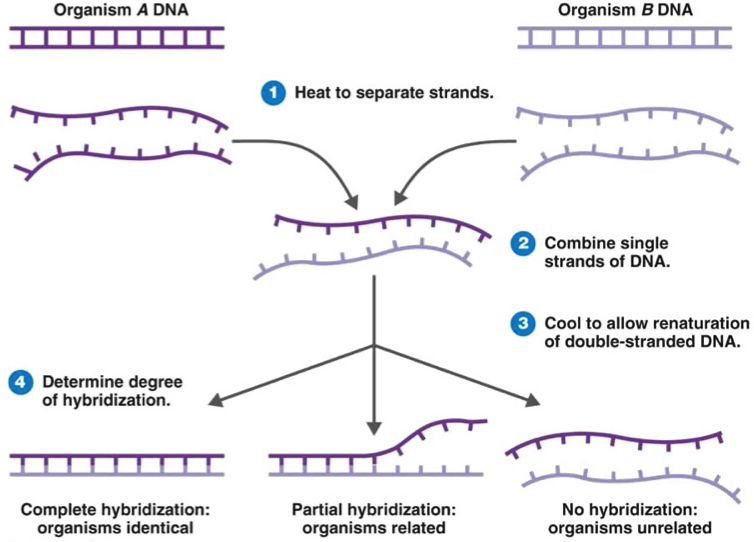
\includegraphics[width=\textwidth]{images/dna-dna_hyb}
  \end{columns}    
  Reassociation of gDNA $\approx$ sequence similarity
\end{frame}

%
\begin{frame}
  \frametitle{DNA-DNA hybridisation (DDH)
  \footnote{\tiny{\href{http://dx.doi.org/10.1016/S0168-6445(00)00040-1
}{Morell\'{o}-Mora \& Amann (2011) \textit{FEMS Microbiol. Rev.} doi:10.1016/S0168-6445(00)00040-1
}}}
  }
  \begin{columns}[T] 
    \column{.5\textwidth} 
      \begin{itemize}
        \item \textcolor{RawSienna}{Find homoduplex $T_{m1}$ for reference $A$}
        \item \textcolor{hutton_green}{Denature gDNA mixture for reference $A$, comparator $B$, and mix}
        \item \textcolor{hutton_green}{Allow gDNA to anneal; hybrids result}
        \item \textcolor{RawSienna}{Find heteroduplex $T_{m2}$ for mixture}
        \item \textcolor{hutton_blue}{$\Delta T_{m} = T_{m1} - T_{m2}$}        
        \item \textcolor{hutton_purple}{High $\Delta T \implies$ genomic difference (fewer H-bonds)}        
      \end{itemize}
    \column{.5\textwidth}
      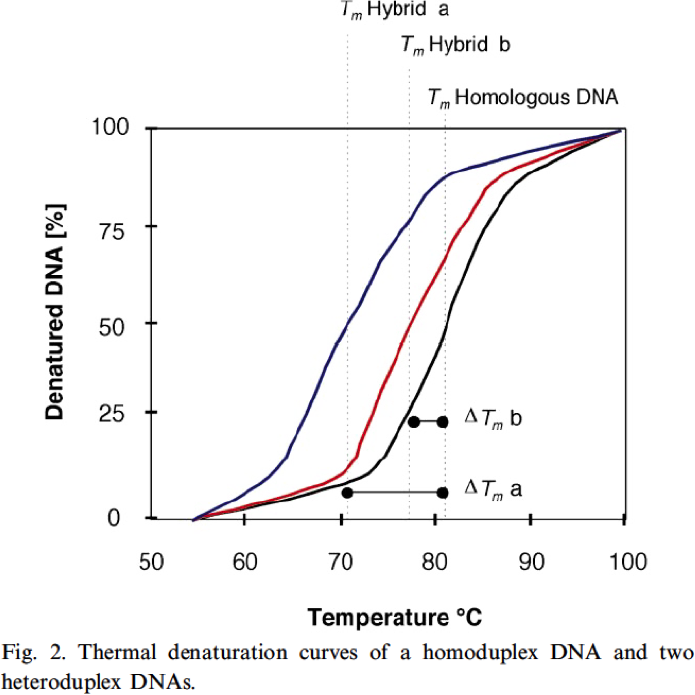
\includegraphics[width=\textwidth]{images/dna-dna_graph} \\
      \textcolor{red}{Proxy for sequence similarity}
  \end{columns}    
\end{frame}

%
\begin{frame}
  \frametitle{DNA-DNA hybridisation (DDH)
  \footnote{\tiny{\href{http://dx.doi.org/10.1007/BF02101980
}{Sibley \& Ahlquist (1984) \textit{J. Mol. Evol.} doi:10.1007/BF02101980
}}}  
  }
  Used for taxonomic classification in prokaryotes since '60s \\
  \textcolor{hutton_green}{Redefined accepted relationships for birds, primates in 1980s} \\
  \textcolor{RawSienna}{Controversial proof that \textit{Homo} shares more recent common ancestor with \textit{Pan} than with \textit{Gorilla}}
  \begin{center}
    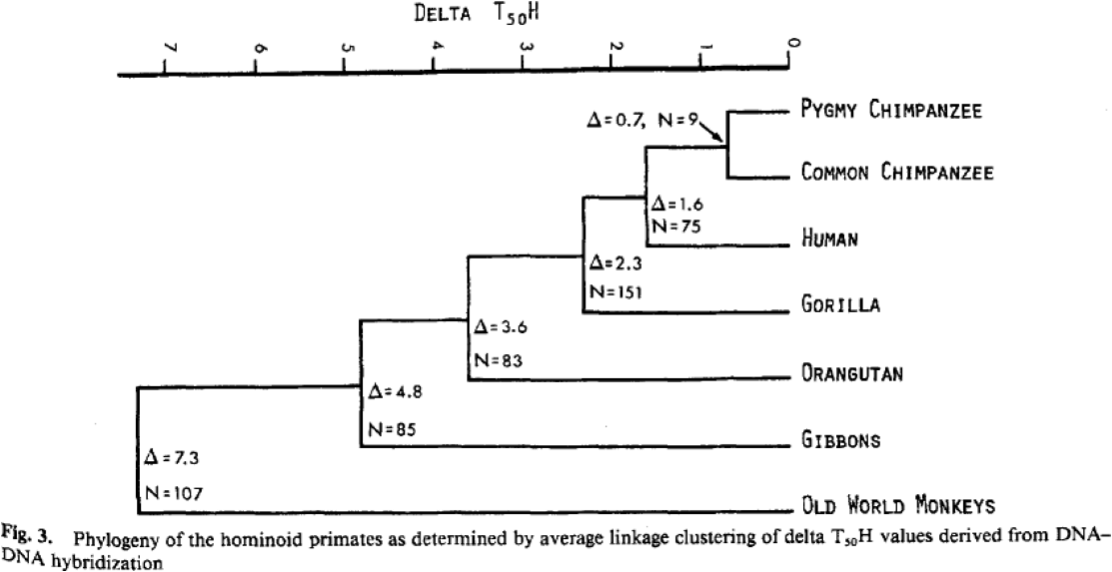
\includegraphics[width=0.9\textwidth]{images/dna-dna_primates} \\
  \end{center}  
\end{frame}

%
\begin{frame}
  \frametitle{DNA-DNA hybridisation (DDH)
  \footnote{\tiny{\href{http://dx.doi.org/10.1007/BF02101980
}{Sibley \& Ahlquist (1984) \textit{J. Mol. Evol.} doi:10.1007/BF02101980
}}}  
  \footnote{\tiny{\href{http://personal.uncc.edu/jmarks/DNAHYB/dnahyb2.html
}{http://personal.uncc.edu/jmarks/DNAHYB/dnahyb2.html
}}}  
  }
  \textcolor{RawSienna}{Controversial proof that \textit{Homo} shares more recent common ancestor with \textit{Pan} than with \textit{Gorilla}} 
  \begin{columns}[T] 
    \column{.6\textwidth} 
      \begin{itemize}
        \item \textcolor{hutton_green}{Allegations of data manipulation (see link $b$)}
        \item \textcolor{hutton_blue}{Close evolutionary relationships difficult to resolve due to $paralogy$}        
        \item \textcolor{hutton_purple}{Still the \textit{de facto} gold standard for microbiological taxonomic classification}        
      \end{itemize}
    \column{.4\textwidth}
      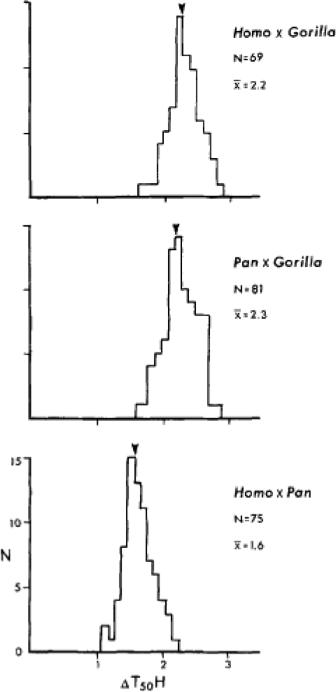
\includegraphics[width=0.6\textwidth]{images/dna-dna_controversy} \\
  \end{columns}    
\end{frame}